\subsection{Применимость существующих решений}

При исследовании существующих решений и анализе их преимуществ и недостатков был сделан вывод о том, что большинство продуктов не подходят для решения поставленной задачи. Однако в данном разделе мы снова возвращаемся к вопросу о применимости существующих решений. Здесь будут более детально рассмотрены два продукта: {\it VBA} и {\it VSTA}. Эти решения стоят особняком, так как первое из них раньше было очень популярно, и по большому счёту отвечало поставленным требованием и действительно могло быть универсальным решением для интеграции в приложения возможностей автоматизации и расширения. В свою очередь {\it VSTA}, по заявлению разработчика --- компании {\it Microsoft}, пришло на смену устаревшему {\it VBA} и формально решает похожие задачи, только для современных приложений и платформ. 

% =======================================================================================================================================
% =======================================================================================================================================

\subsubsection{VBA}

Как уже обсуждалось ранее, реальный проект, в рамках которого и возникла задача разработки платформы для автоматизации и расширения приложений, подразумевал портирование устаревшего приложения на современные языки и платформы. В <<старом>> приложении для автоматизации и расширения как раз и использовался {\it VBA}. Данное решение обладало многими преимуществами:
\begin{itemize}
\item простота интеграции в основное приложение;
\item наличие удобной среды разработки;
\item наличие отладчика;
\item наличие инструментов для сохранения и загрузки проектов;
\item возможность использовать доступные в операционной системе {\it COM}  объекты и {\it ActiveX} компоненты;
\item простота реализации взаимодействия основного приложения и расширения.
\end{itemize}

Исходя из перечисленных особенностей, можно сделать вывод, что для <<старого>> приложение решение с {\it VBA} было оптимальным. Однако по ряду причин невозможно использовать {\it VBA} в современном приложении не {\it .NET}:

\begin{itemize}
   \item {\it VBA} не совместим с {\it .NET};
   \item нет поддержки 64-битных приложений;
   \item {\it VBA} является устаревшей и не поддерживается.
\end{itemize}

% =======================================================================================================================================
% =======================================================================================================================================

\subsubsection{VSTA}

При теоретическом исследовании возможностей {\it VSTA} не было выявлено явного несоответствия требованиям, сформулированным в рамках реализуемого в компании проекта. Многие проблемы были выявлены уже позже. Часть из них проявилось на этапе разработки и была таки или иначе исправлена, часть была выявлена лишь на этапе финального тестирования. Однако вцелом {\it VSTA} решает нужные задачи, и так или иначе это решение было внедрено. Ниже в общих чертах будут описаны детали реализации, возникшие трудности и пути их решения.

В терминах {\it VSTA} основное приложение, которое будет расширяться за счёт макросов, называется хост-приложением. Хост-приложение должно быть специальным образом зарегистрировано. Фактически, регистрация сводится к созданию нескольких ключей реестра {\it Windows}. Для этого был написан скрипт, в дальнейшем встроенный в инсталлятор готового продукта. Для работы с {\it VSTA}-студией в хост-приложении есть объект типа {\tt EnvDTE.DTE}, через который можно получать доступ ко всем объектам {\it VSTA}-редактора и подписаться на необходимые события.

{\it VSTA}-макросы могут работать в двух режимах – runtime и design. Идея runtime-режима заключается в том, что макрос выполняется в отдельном (от хост-приложения) процессе, доступ к объектам хост-приложения осуществляется через соответствующие прокси-объекты. В design-режиме наоборот: макрос выполняется в том же процессе, что и хост-приложение, доступ к объектам основного приложение осуществляется напрямую. Использование runtime-режима в некотором смысле безопаснее, однако использование прокси-объекта, во-первых, влияет на производительность, а во-вторых, накладывает ряд ограничений. Например, нельзя создавать объекты хост-приложения <<напрямую>>, используя оператор {\tt new}. В результате для использования на проекте был выбран design-режим.

На рисунке \ref{diagram_vsta_1} показана общая схема взаимодействия основного приложения и {\it VSTA}. 

\begin{figure}[!h]
    \centering
    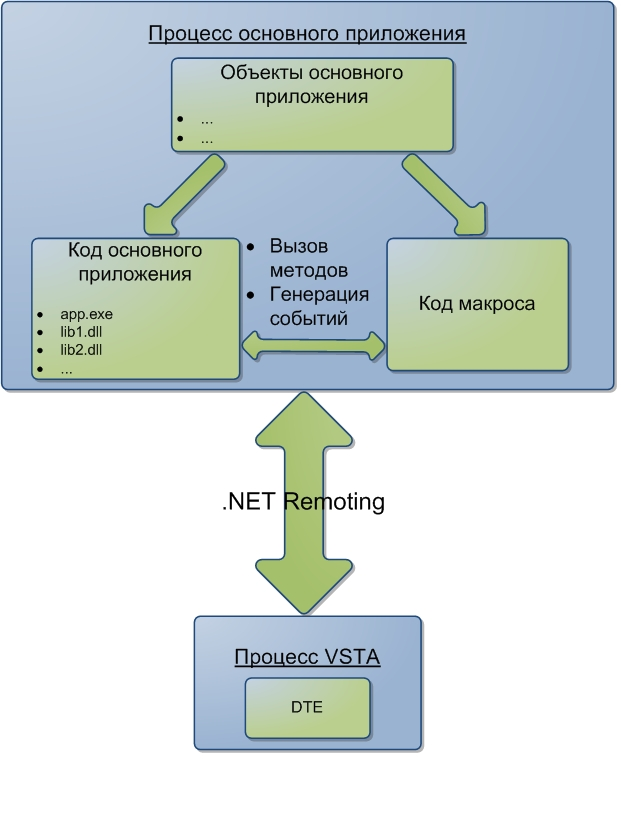
\includegraphics[width=10cm]{diagram_vsta_1.jpg}
    \caption{Взаимодействие основного приложения и VSTA}
    \label{diagram_vsta_1}
\end{figure} 

Как уже обсуждалось ранее, в предложенном решении макрос выполняется в том же процессе, что и остальное приложение. Отдельный процесс {\tt VSTA.EXE} –-- это сама {\it VSTA}-студия (т.е. приложение, в котором производится редактирование кода макроса и отладка). 
В отличие от {\it VBA}, макросы {\it VSTA} не интерпретируются, а компилируются. Это значит, что после внесения изменений в код макроса он должен быть скомпилирован, а полученный бинарный код подгружен хост-приложением. Скомпилировать макрос можно через меню {\it VSTA}-студии. Помимо этого, для удобства автоматическая компиляция и перезагрузка кода происходит при каждом сохранении макроса. Более того, если в момент сохранения макрос не компилировался (к примеру, там были синтаксические ошибки), пользователю будет показано диагностическое сообщение.

С точки зрения {\it .NET}, скомпилированный код макроса является обычной managed-сборкой (фактически это файл с расширением {\tt .dll}). Такая сборка подгружается в домен приложения в помощью {\it .NET Reflection}. После загрузки происходит присваивание всех нужных объектов (опять же, с помощью {\it Reflection}), подписка на события. 

Важно отметить, что макро-проект может ссылаться на любую другую managed-сборку. Это значит, что, во-первых, в макросах можно использовать всю мощь библиотек .NET и, возможно, сторонних проектов, а во-вторых, макрос может использовать объекты и код основного приложения. Таким образом, из макроса можно запросить любой singleton-объект приложения, и это будет тот же экземпляр класса, который используется хост-приложением. Это весьма удобно и открывает широкие возможности перед разработчиком макроса.

Для повторения функциональности, предоставляемой {\it VBA}, было необходимо вручную (но с использованием средств и механизмов, предоставляемых {\it VBA}) реализовывать некоторые дополнительные возможности:
\begin{itemize}
\item предоставление доступа к объектам основного приложения;
\item генерация и обработка событий;
\item отладка.
\end{itemize}
Реализация данных возможностей --- сугубо техническая задача, поэтому детали в рамках данной главы не рассматриваются. Но стоит отметить, что из-за внутренних ошибок и проблем {\it VSTA} иногда приходилось разрабатывать обходные решения. При некоторой последовательности действий, которую легко воспроизвести, {\it VSTA} могла зависать либо аварийно завершаться.

{\bf Выводы.} В целом, {\it VSTA} подходит для решения поставленной задачи. Ниже описаны основные сложности:
\begin{itemize}
\item {\it VSTA}, несмотря на то, что последний релиз имеет версию 2.0, ещё несколько <<сыровата>>: далеко не все возможности работают именно так, как заявлено разработчиками. В самой среде довольно много ошибок, приводящих к зависанию или аварийной остановке {\it VSTA}.
\item отсутствует полноценная документация;
\item процесс интеграции с основным приложением более сложный и трудоёмкий (и не такой автоматизированный) как в случае с {\it VBA}.
\end{itemize}

Помимо этого, есть ещё одна проблема, выявленная уже после завершения работы над продуктом:
\begin{itemize}
\item {\it Microsoft} перестала поддерживать {\it VSTA 2.0}. Более того, нет конкретной информации о том, будут ли выпускаться новые версии. На настоящий момент невозможно приобрести лицензию (а значит и использовать в коммерческих целях) на {\it VSTA}.
\end{itemize}
Судя по всему данная проблема решения не имеет. Это и стало <<последней каплей>>, чтобы принять решение самостоятельно разрабатывать платформу для интеграции возможностей автоматизации и расширения в приложения.